\documentclass{article}
\usepackage[utf8]{inputenc}
\usepackage[margin=1.25in]{geometry}
\usepackage{tikz}
\usetikzlibrary{shapes.geometric}
\usepackage{pgfplots}
\usepackage{graphicx}
\graphicspath{ {images/} }

\begin{document}

Responses to the Referee

\vspace{12pt}

I thank the referee for the very helpful comments on my paper. They are insightful and, by addressing them, I am certain my paper will be easier to read, more refined, and have a clearer marginal contribution to the literature. I now included the blind referee in the acknowledgements. The referee has raised four points and I intend to address one at a time by showing specifically which changes I've made to the text to try to accommodate the recommendations. \textbf{Changes or additions are in bold}.

\begin{enumerate}
    \item \textit{"THERE IS A GENERAL LACK OF CONNECTION TO THE PREVIOUS LITERATURE, ESPECIALLY IN THE INTRODUCTION. ALMOST NO REFERENCES ARE GIVEN AND AS A RESULT THE PAPER IS NOT WELL POSITIONED. THIS MAKES IT HARD TO DETERMINE THE MARGINAL CONTRIBUTION."}
    
    I agree that the paper doesn't do a long literature review. I tried to expand on that by making the geography-institutions debate a little bit more nuanced:
    
    \begin{quote}
        Since Acemoglu, Johnson and Robinson's (2001) seminal paper supporting the link between institutions and development, the debate over the role in institutions on economic growth has spurred much research. Those who are critic of institutionalism are perhaps better represented by Jeffrey Sachs (2003) \textbf{and some of his co-authors}, who have emphasized the prevalence of ecology and geography over institutions in economic development. \textbf{Others, like Nunn and Puga (2012), have taken a more nuanced position on this split, by arguing that geography has historically played a key role in shaping institutions and thus can indirectly explain income differences between countries}.
    \end{quote}
    \begin{quote}
        In spite of the very prolific work on this field, most of the literature has resorted to microeconometric techniques in testing hypotheses. There are several reasons for that. The most important one is that complete time series of country-wide institutional quality indicators have only become available in the last fifteen years. This has limited the extent to which researchers can explore dynamics in the institutions-growth relationship since the data are still too scant for individual-country time-series analysis. \textbf{Additionally, although the popularity of  panel vector autoregressions has been increasing since the seminal work of Holtz-Eakin \textit{et al} (1988), its use is still remarkably rarer than traditional VARs.}
    \end{quote}
    
    Additionally, I mentioned some earlier literature that applied macroeconometric techniques to this question and tried to explain how I expanded on their work and what is the most important marginal contribution of the paper:

    \begin{quote}    
        \textbf{Like Chong and Calderón (2000), who show evidence of bi-directional Granger causality between institutions and growth, I take a macroeconometric approach to this debate. I extend their insight by building a Panel Structural Vector Autoregression (SVAR) model for 119 countries over 10 years using Arellano-Bond's dynamic panel equations. The largest contribution of this approach is showing that institutions and growth have a \textit{dynamic and bi-directional} relationship and providing reliable estimates of it. While most of the literature usually focuses on how institutions help explain differences \textit{between countries} over the very long run, results here presented show how and to which extent, on average, changes in institutions over time help explain changes in income \textit{within} the same country.}
    \end{quote}

    
    \item \textit{"THIS IS WHERE YOU DISCUSS THE ARELLANO-BOND IV APPROACH. THIS APPROACH IS USUALLY APPLIED IN THE UNIVARIATE SETTING AND SO AS A READER I WOULD BE INTERESTED TO KNOW IF THERE ARE ANY PROBLEMS TO EXTENDING IT TO THE CURRENT MULTIVARIATE SETTING."}
    
    I expanded \textit{footnote 2} to address this issue directly, referring to the literature that details this exact point and briefly explaining the intuition behind expanding GMM dynamic panels to a multivariate framework:
    
    \begin{quote}
        As described in Arellano and Bond (1991), the GMM estimators assume $E[e_{m,i,t}|Z] = 0$, where $Z$ is a matrix of instruments which are correlated with regressors and orthogonal to the error terms. For each equation, the moment estimators will minimize the above assumption by changing the symmetric matrix $M$ in $[(X'ZMZ'X')^{-1}X'ZMZ'Y']$, where $X$ is a matrix of all lagged variables on the right hand-side and $Y$ is a vector of the variable on the left-hand side. \textbf{Bond (2002) shows that GMM estimators for autoregressive models, including Arellano-Bond, extend in a natural way to include "a vector of current and lagged values of additional explanatory variables". Even if regressors are endogenous and correlated with the contemporaneous residuals, lagged regressors are efficient instruments that can be included in $Z$}.
    \end{quote}
        
    \item \textit{EQN. (2): THIS MODEL IS STATED IN DIFFERENCES AND WITHOUT ANY ERROR CORRECTING TERMS WITHOUT ANY JUSTIFICATION. THIS IS NOT GOOD ENOUGH.}
    
    First-differencing and lagged instruments were used, in the Arellano-Bond framework, to get to a consistent estimate of the parameters. Perhaps I was not clear enough and it looked as if I was trying to build an error correction model with potentially cointegrated variables. I added a phrase to clarify that and made the strategy more clear.
    
    \begin{quote}
        However, since $f_i$ is correlated to the error terms, estimation through OLS leads to biased coefficients. \textbf{As explained in Baltagi (2008), first-differencing and using lagged instruments is a good strategy to get consistent parameters and eliminate individual fixed-effects when $N$ is large and $T$ is fixed. Following that line, I estimate a system of $m = 2$ equations with Arellano-Bond's GMM/IV technique}. Each equation in the system has the first difference of an endogenous variable on the left hand side, $p$ lagged first differences of all $m$ endogenous variables on the right hand side\textbf{ and no constant}.
    \end{quote}

    \item \textit{"HERE YOU SAY THAT THE SHOCKS ARE IDENTIFIED USING CHOLESKY FACTORIZATION. ANY REASONS FOR THIS? AND WHAT ABOUT THE ORDERING OF THE VARIABLES? THIS HAS TO BE MOTIVATED TOO."}
    
    Cholesky factorization became the standard workhorse in the VAR literature. However, I agree that there was a lack of motivation on why I chose to present just one ordering. As argued in the methodology section, I think the baseline ordering is more "robust" under the following rationale: "Since I'm trying to test the institutions hypothesis, I should choose as baseline whatever ordering with the smallest impact of institutions on income." However, I agree that there is no \textit{strong} reasons why institutions shouldn't impact income contemporaneously and decided to present the results with the alternative ordering in the robustness section. I added a line to the methodology section:
    
    \begin{quote}
        To identify the model I need to impose one restriction to orthogonalize the contemporaneous responses. In the Cholesky ordering, institutional quality is set to have no contemporaneous effect on GDP per capita while the latter is allowed to contemporaneously impact the former. By construction, this \textbf{reduces} the short-term impact of institutional quality on GDP per capita, so this design is more robust if one is trying to test the institutional hypothesis. \textbf{However, in the absence of strong \textit{a priori} reasons why institutions should not affect income contemporaneously, I present the results using the alternative ordering of variables in the robustness section.}
    \end{quote}
    
    And a paragraph with the respective charts to the robustness section:

    \begin{quote}
        \textbf{I test the robustness of the results with two alternative specifications. First, I invert the Cholesky ordering of endogenous variables. The baseline specification restricts  contemporaneous effects of institutions on income, while the alternative specification does the inverse. Since those variables are contemporaneously correlated, restrictions will tend to limit the positive impact of a variable on the other. As expected, the alternative specification shows a higher peak response of income to institutional quality (1.9\% vs. 1.7\% in the baseline) and a lower peak response of institutional quality to income (0.2\% vs. 0.3\% in the baseline). Such small differences do not change the overall interpretation of results. [...]}        
        \begin{figure}[ht]
        \begin{center}
            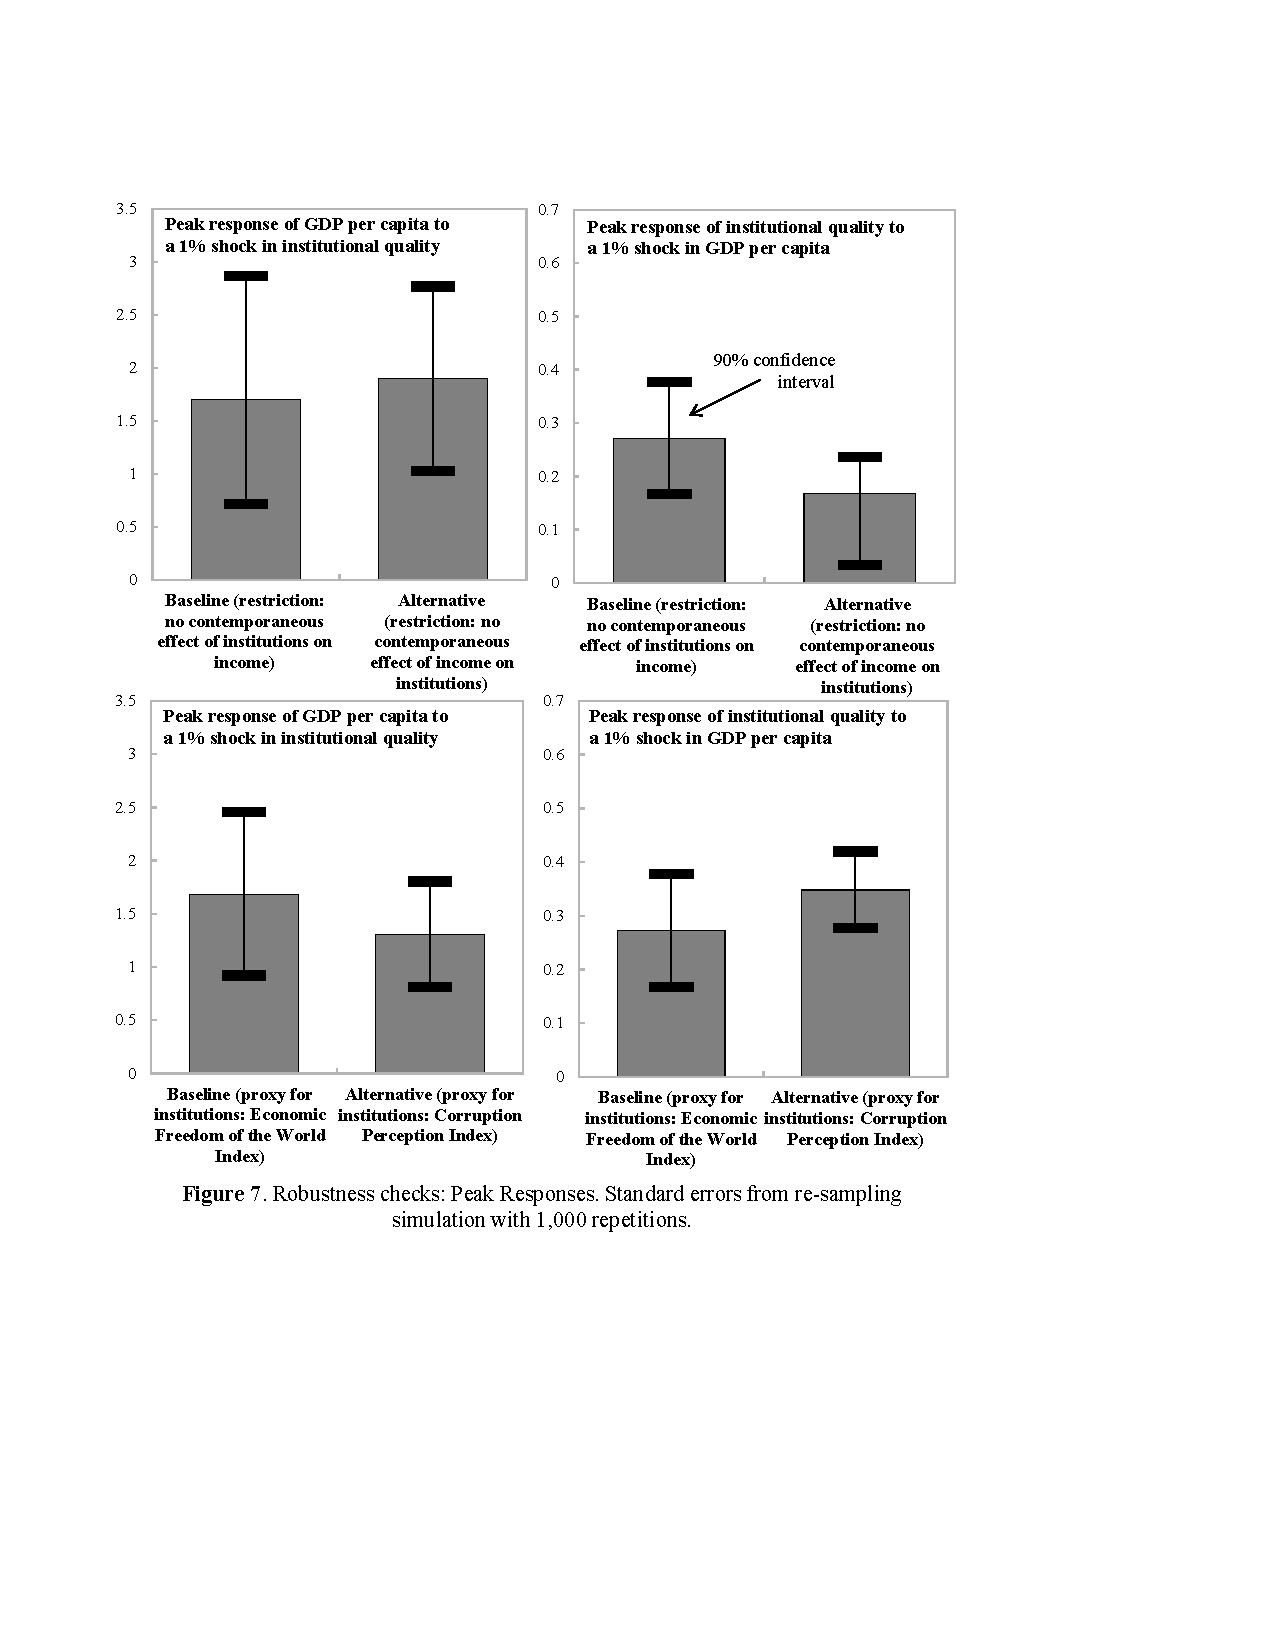
\includegraphics[scale=0.7]{robustness.pdf}
        \end{center}
        \end{figure}
    \end{quote}

    
\end{enumerate}


\end{document}
